\section{Diagrama de Objetivos (1.2)}

\subsection{Descripci\'on: Sufragio}


Llega un votante a la mesa. En caso de tener alguna discapacidad, tiene prioridad en la cola. 

Si el votante lo necesitase, podrá requerir ayuda y/o auriculares al presidente de mesa quien se deberá contactar con el Fiscal General con el fin de conseguir los auriculares. Para personas que posean problemas de movilidad, se les permitirá imprimir su voto en máquinas ubicadas en planta baja, mientras que el presidente de mesa les acercará la urna, para que pueda depositar su boleta al finalizar el sufragio. Sólo usará la máquina impresora de voto de la misma, mientras que es responsabilidad del presidente de mesa acercar la urna para que su voto sea contabilizado en la mesa que le corresponde por el padrón.

En el caso de que no posea una discapacidad, espera en la cola de votación de la mesa. 
En ambos casos, cuando es su turno, el votante le entrega su DNI al presidente de mesa. Este verifica su identidad al asegurarse que la persona que le entregó el DNI es la poseedora del mismo, que se encuentra en el padrón correspondiente a la mesa, y que no votó todavía. Los fiscales de mesa hacen lo mismo. Si hay algún problema, el presidente de mesa y/o los fiscales notifican al fiscal general de la escuela. El mismo decidirá si la persona está apta para emitir voto o no.\\

Si el votante pasa la verificación, el presidente de mesa procede a entregarle la boleta y le retiene el DNI. A la boleta entregada, le quita un troquel que posee el código identificatorio, dejándola con el otro código idéntico en la boleta.
Luego, el votante se acerca la máquina impresora de voto e inserta la boleta.\\

Entonces, el sistema de la máquina muestra por pantalla las opciones de votar por categoría o votar lista completa. Para ambos casos, se presentan las opciones (se incluye también la de voto en blanco) en posiciones aleatorias en la pantalla.

El votante podrá entonces elegir entre las opciones y al finalizar, obtener la boleta con su voto impreso (tanto en el papel como en el chip). El votante puede verificar en la máquina que lo impreso en el chip sea correcto.\\

Luego, el votante quita el troquel restante a la boleta, se lo entrega al presidente de mesa y si coincide con el retirado previamente, puede pasar a depositar la boleta en la urna siempre y cuando no haya cantado cuál será su voto. Si el votante canta su voto, la boleta quedará anulada impidiéndole ingresarla en la urna. 

Si el votante se arrepiente, puede pedir otra boleta y repetir el proceso.
Finalmente, el presidente de mesa le hace firmar al votante el padrón, y le devuelve el DNI conjunto a la constancia de voto.\\

En el caso de que falle alguna máquina, se pueden reemplazar por las dos de repuesto que posee cada escuela las cuales estarán a cargo del fiscal general. Si en una escuela dejan de funcionar más de dos máquinas, se podrá compartir la maquina de sufragio entre mesas, pero cada boleta deberá ser depositada en la urna correspondiente.\\
\textcolor{red}{El fiscal general puede, en todo momento, utilizar el pendrive suministrado por el Ministerio, para chequear que el código que se ejecuta en cada máquina, es el correcto.}

Pasadas las 18hs, las fuerzas de seguridad cierran las puertas de las escuelas. Y una vez terminados los comicios, empieza el conteo.

\newpage
\subsection{Diagrama}

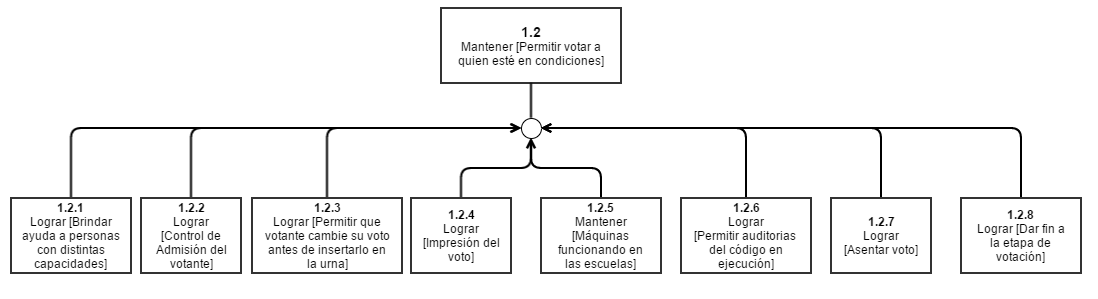
\includegraphics[scale=0.45]{imagenes/Diagramas/12/12.png}
\\
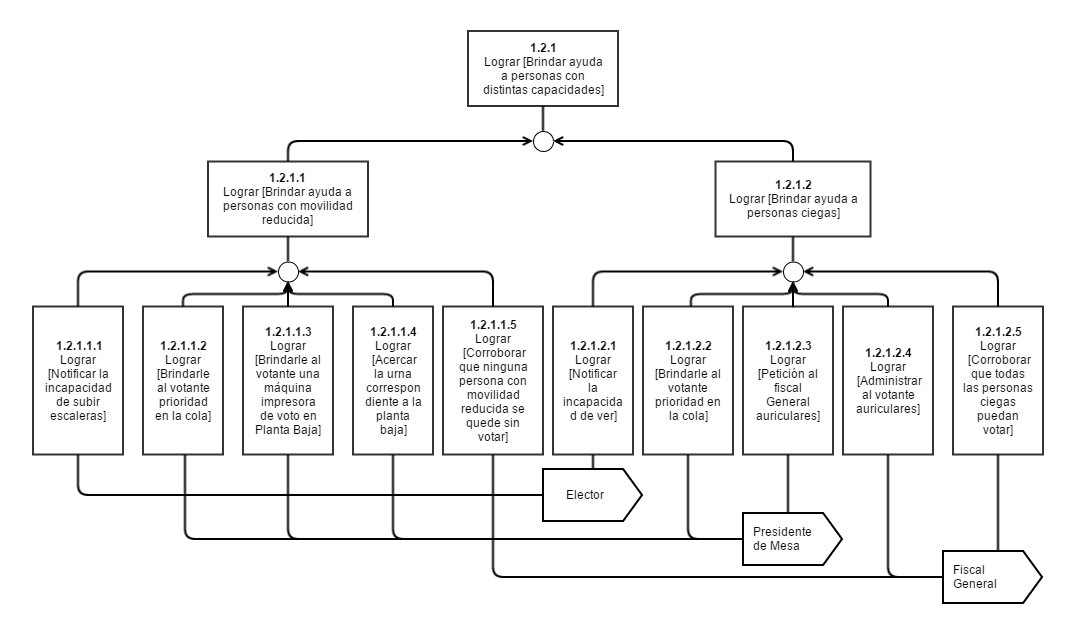
\includegraphics[scale=0.55]{imagenes/Diagramas/12/121.png}
\\
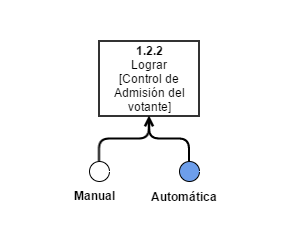
\includegraphics[scale=0.55]{imagenes/Diagramas/12/122.png}
\\
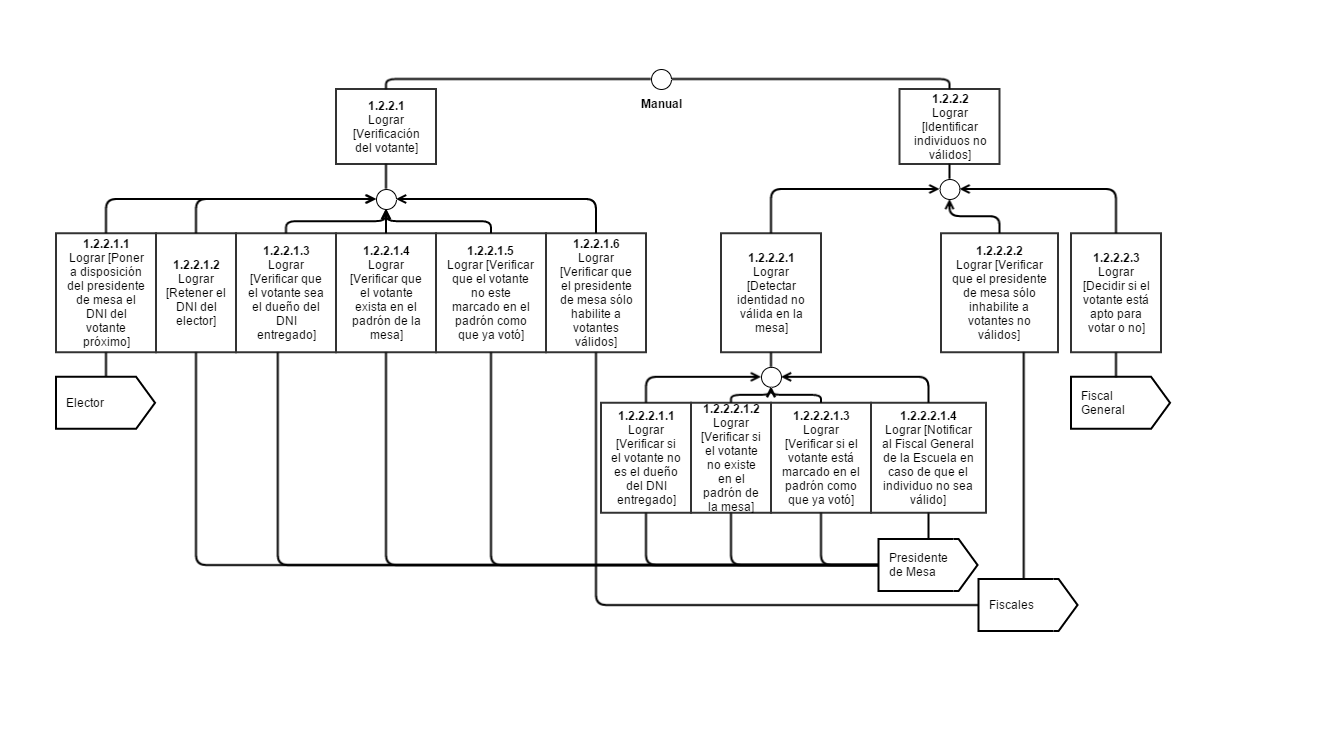
\includegraphics[scale=0.55]{imagenes/Diagramas/12/122a.png}
\\
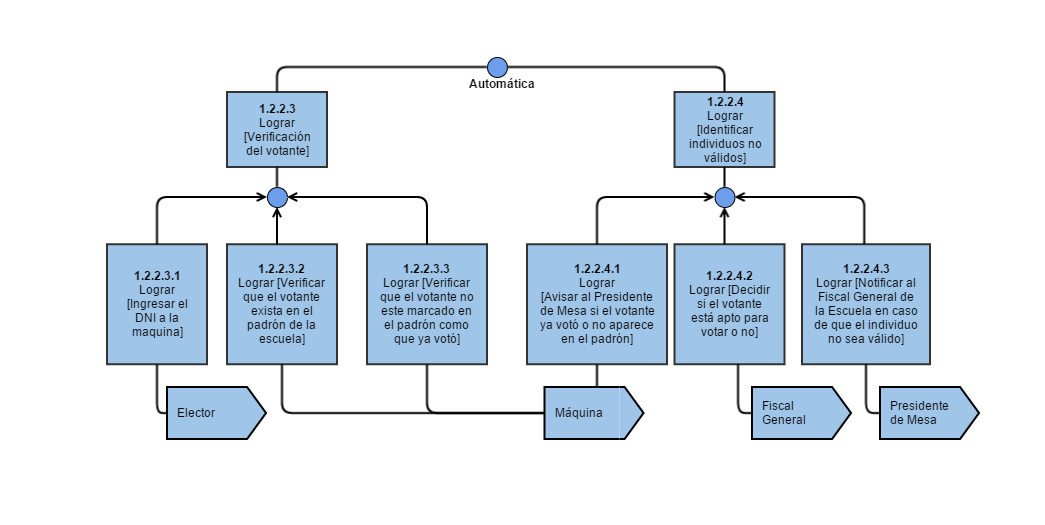
\includegraphics[scale=0.55]{imagenes/Diagramas/12/122b.png}
\\
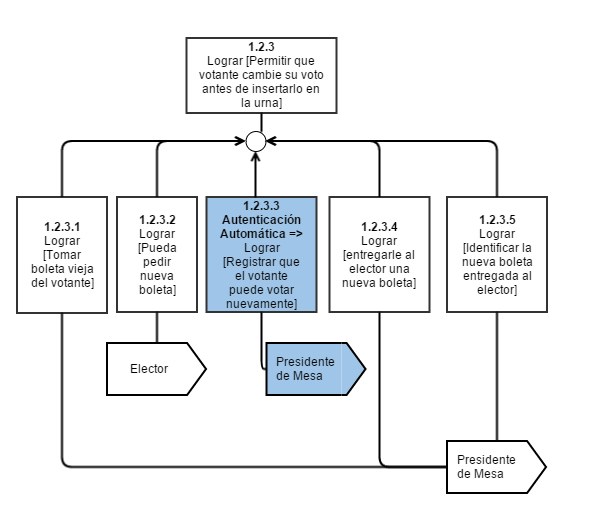
\includegraphics[scale=0.55]{imagenes/Diagramas/12/123.png}
\\
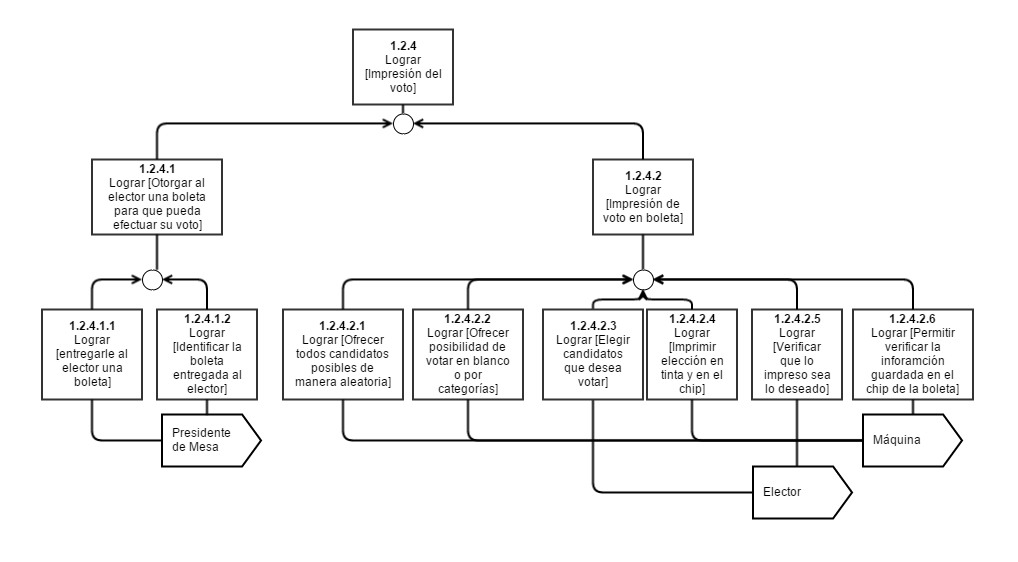
\includegraphics[scale=0.55]{imagenes/Diagramas/12/124.png}
\\
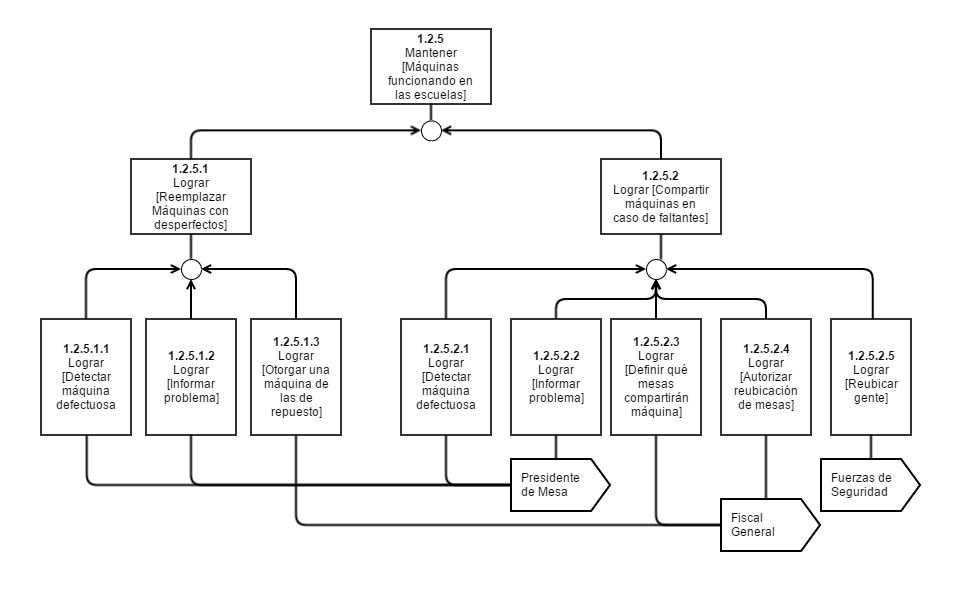
\includegraphics[scale=0.55]{imagenes/Diagramas/12/125.png}
\\
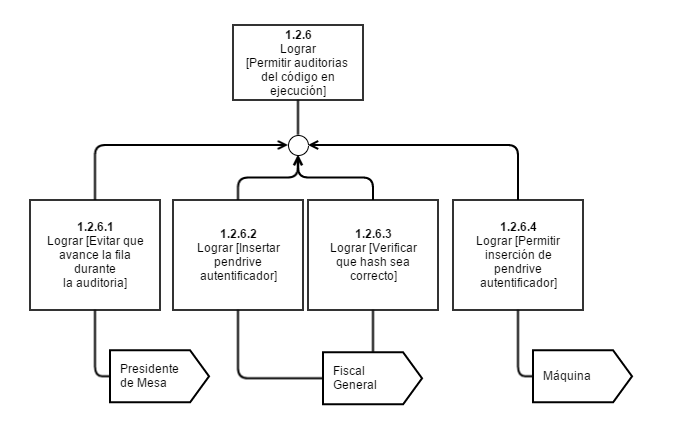
\includegraphics[scale=0.55]{imagenes/Diagramas/12/126.png}
\\
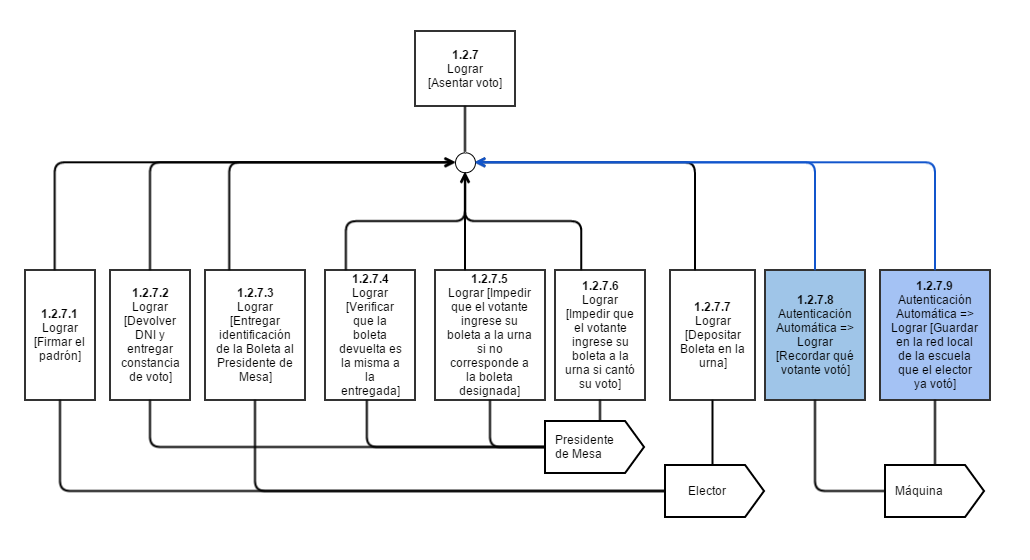
\includegraphics[scale=0.55]{imagenes/Diagramas/12/127.png}
\\
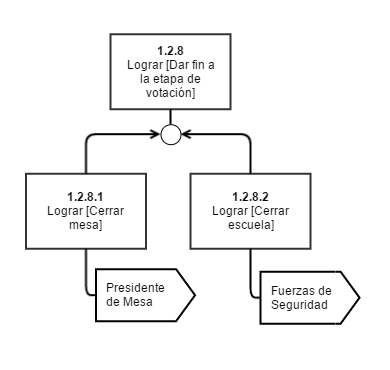
\includegraphics[scale=0.55]{imagenes/Diagramas/12/128.png}


\newpage
\subsection{Lista de requerimientos}

\begin{itemize}
\item Ofrecer todos los candidatos posibles de manera aleatoria
\item Ofrecer votar en blanco o en categorias
\item Imprimir elecciones en el chip y en tinta
\item Permitir la verificación de la información guardada en el chip
\item Permitir inserción de pendrive autentificador
\end{itemize}